\documentclass[../main]{subfiles}
\begin{document}

\graphicspath{{../figures/}}

\section{提案手法}





\subsection{提案手法の概要}
本研究では,移動ロボットにマイクを搭載し,自己位置の座標ごとに聞こえる音を予測し,それらの差分から異常音源の座標を推定する手法を提案する.
学習時には,異常音源を含まない経路でロボットを走行させ,正常時の座標と音の関係をモデルに学習させる.
運用時には,学習したモデルを用いて検査対象となる経路を走行させ,閾値処理により経路内の異常音源の有無を判別したのち,異常音源が確認された場合には,その座標を推定する.
フローチャートを\reffig{flowchart}に示す.
\begin{figure}[tb]
  \centering
  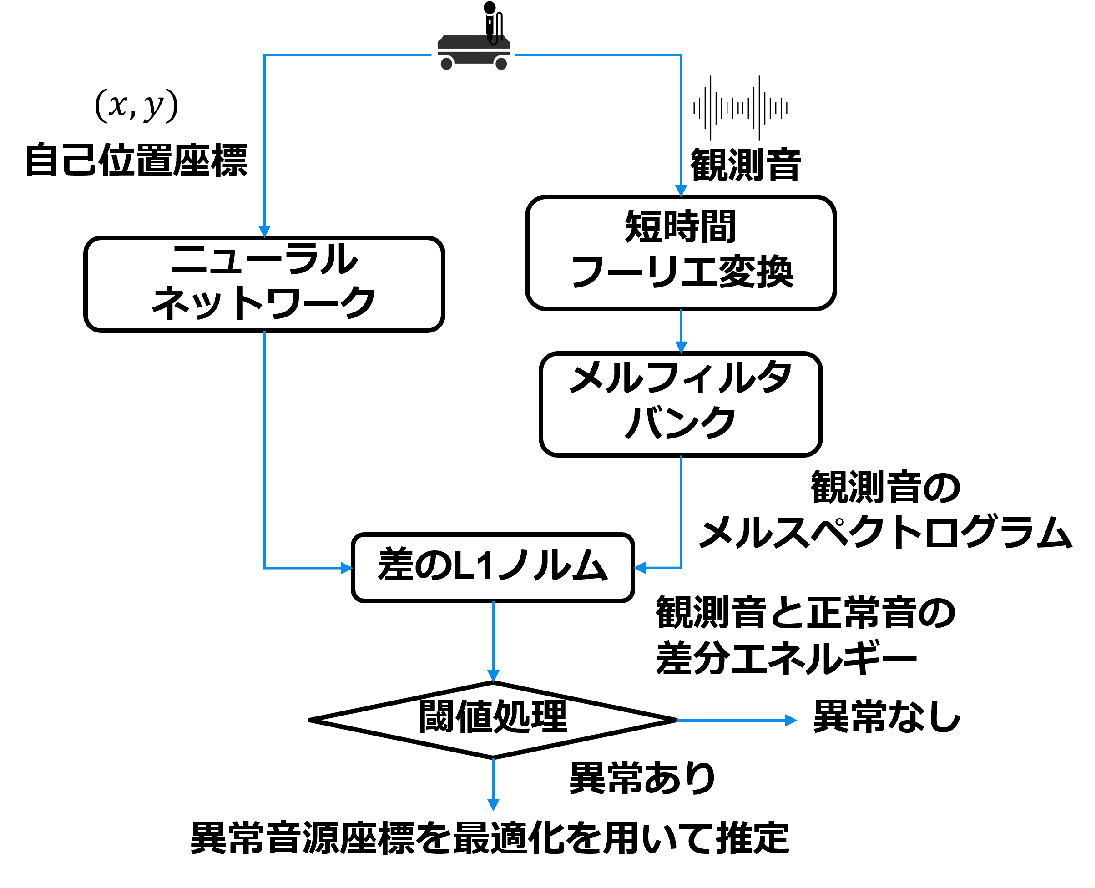
\includegraphics[keepaspectratio, width=0.8\linewidth]{flowchart.pdf}
  \caption{提案手法のフローチャート}
  \labfig{flowchart}
\end{figure}
\subsection{ニューラルネットワークによる正常音のマッピング}
ニューラルネットワークとは,人間の脳の神経細胞を模倣した計算モデルであり,入力層,中間層,出力層から構成され,
各層のノード間の結合には重みが設定されている.
これらの重みを学習することで,入力データから出力データを予測するモデルを構築することができる.
本研究では,ニューラルネットワークを用いて,自己位置の座標を入力とし,その座標に対応する正常音を出力するモデルを構築する.
\subsection{SAM optimizer}
SAM optimizerは,Sharpness-Aware Minimizationの略であり,モデルの汎化性能を向上させるための最適化手法である.
SAM optimizerは,モデルの重みの更新時に,重みの変化に対する損失関数の変化が小さくなるように重みの更新を行うことで,
汎化性能を向上させることを目的とした最適化手法である.
本研究では,音のマッピングを行うことをコンセプトとして挙げており,座標の変化に対して出力である音の変化が滑らかになるように,
モデルの学習を行うために,SAM Optimizerを用いる.
\subsection{短時間フーリエ変換}
本研究では,座標ごとに聞こえる音をマッピングすることをコンセプトとしているが,音圧のデータは時間ずれの影響を非常に受けやすいことから,音圧の時系列データから
定常的な特徴量を抽出する必要がある.
そのため,音圧の時系列データから短時間フーリエ変換を行い,更にメルフィルタバンクの処理を適用し,次元を削減したメルスペクトログラムを特徴量として用いる.
\subsection{異常音座標の推定}
本研究では、音のエネルギーが距離の二乗に反比例して減衰するという前提のもと,最適化手法を用いて異常音源の座標を推定する.
コスト関数を,異常音源の座標と,ロボットの自己位置座標間の距離の-2乗に比例定数をかけたものと,正常音と観測音のメルスペクトログラムの差分によって得られるエネルギーの差に設定し,
変数として自己位置座標と比例定数を最適化する.

\begin{equation}
  \underset{\mathbf{x_a}, \alpha}{\arg\min} \sum \left| L_1 (\mathbf{m_i^o}, \mathbf{m_i^n})^2 - \frac{\alpha}{L_2 (\mathbf{x_i}, \mathbf{x_a})^2} \right|
\end{equation}

\end{document}
